\documentclass[a4paper,12pt,openany]{book}


\usepackage[T1,plmath]{polski} % lepiej to zamiast babel!
\usepackage[utf8]{inputenc} % w razie kłopotów spróbować: \usepackage[utf8x]{inputenc}
\usepackage{fancyhdr} % nagłówki i stopki
\usepackage{indentfirst} % WAŻNE, MA BYĆ!
\usepackage[pdftex]{graphicx} % to do wstawiania rysunków
\usepackage{amsfonts} % pakiety od AMS, ułatwiają składanie pewnych techniczno---matematcyznych rzeczy
\usepackage{amsmath} % to do dodatkowych symboli, przydatne
\usepackage{amssymb} % to też do dodatkowych symboli, też przydatne
\usepackage{amsthm}
\usepackage{enumitem}
\usepackage[pdftex,
            left=1.1in,right=1.1in,
            top=1.1in,bottom=1.1in]{geometry} % marginesy
\usepackage{float}
\usepackage[font=small,labelfont=bf]{caption}

\usepackage[colorlinks=true]{hyperref} % odnośniki interaktywne w PDFie
\hypersetup{allcolors=black}

\usepackage{listings}
\lstset{
    basicstyle=\footnotesize\tt,
    numbers=left,
    numberstyle=\tiny,
    frame=tb,
    tabsize=4,
    columns=fixed,
    showstringspaces=false,
    showtabs=false,
    keepspaces,
    commentstyle=\color{black},
    keywordstyle=\color{black}
}
\newfloat{lstfloat}{htbp}{lolst}[chapter]
\floatname{lstfloat}{Listing}
\def\lstfloatautorefname{Listing}

% jesli potrzeb, można oczywiście wstawić inne pakiety i swoje definicje...



% definicje nagłówków i stopek
\pagestyle{fancy}
\renewcommand{\chaptermark}[1]{\markboth{#1}{}}
\renewcommand{\sectionmark}[1]{\markright{\thesection\ #1}}
\fancyhf{}
\fancyhead[LE,RO]{\footnotesize\bfseries\thepage}
\fancyhead[LO]{\footnotesize\rightmark}
\fancyhead[RE]{\footnotesize\leftmark}
\renewcommand{\headrulewidth}{0.5pt}
\renewcommand{\footrulewidth}{0pt}
\addtolength{\headheight}{1.5pt}
\fancypagestyle{plain}{\fancyhead{}\cfoot{\footnotesize\bfseries\thepage}\renewcommand{\headrulewidth}{0pt}}


% interlinia
\linespread{1.25}
\sloppy



\begin{document}
\begin{titlepage}
% ~

\begin{tabular}{c@{\hspace{21mm}}|@{\hspace{5mm}}l}
\vspace{---20mm} & \\
\multicolumn{2}{l}{\hspace{---12.5mm} 
\includegraphics[width=8cm]{LogoUMCS.jpg}} \\
\multicolumn{2}{@{\hspace{20mm}}l}{\vspace{---4mm}} \\
\multicolumn{2}{@{\hspace{28mm}}l}{\Large \sf UNIWERSYTET MARII
	CURIE-SKŁODOWSKIEJ} \\
\multicolumn{2}{@{\hspace{28mm}}l}{\vspace{---4mm}} \\
\multicolumn{2}{@{\hspace{28mm}}l}{\Large \sf W LUBLINIE} \\
\multicolumn{2}{@{\hspace{28mm}}l}{\vspace{---4mm}} \\
\multicolumn{2}{@{\hspace{28mm}}l}{\Large \sf Wydział Matematyki, Fizyki i
	Informatyki} \\
\multicolumn{2}{@{\hspace{28mm}}l}{\vspace{21mm}} \\
& {\sf Kierunek: \textbf{informatyka} } \\
%& {\sf Specjalność: \textbf{informatyczna}} \\ % wpisujemy tylko jeśli jest!!!
& \\\\\\
& {\sf \large \bfseries Kamil Goławski} \\
& {\sf nr albumu: 312304} \\
& \\\\\\
& \Large \sf \bfseries Projektowanie oraz implementacja\\
& \Large \sf \bfseries wielowarstwowego Rest API w Spring Boot\\
& \Large \sf \bfseries — od CRUDa do modularnego systemu\\
& \Large \sf \bfseries zarządzania danymi pogodowymi \\\\[---10pt]
& {\large \sf Designing and implementing\\
& {\large \sf a multi-layer Rest API in Spring Boot}\\
& {\large \sf — from CRUD to a modular\\
& {\large \sf weather data management system\\
& \\
& \\
& \\
& {\sf Praca licencjacka}  \\
& \vspace{---7mm} \\
&  {\sf napisana w Katedrze oprogramowania systemów informatycznych} \\
&  {\sf Instytutu Informatyki UMCS} \\
& \vspace{---7mm} \\
& {\sf pod kierunkiem \bfseries dr hab. Beaty Byliny} \\
\multicolumn{2}{@{\hspace{28mm}}l}{\vspace{15mm}} \\
\multicolumn{2}{@{\hspace{28mm}}l}{\textbf{\textsf{Lublin 2025}}}
\end{tabular}
\end{titlepage}


\tableofcontents{}

\chapter*{Wstęp} % z gwiazdką, więc bez numerka...
\addcontentsline{toc}{chapter}{Wstęp} % ...ale w spisie treści ma być...
\chaptermark{Wstęp} % ...i w paginie górnej

W dobie postępu technologicznego, inżynieria oprogramowania zmierza ku tworzeniu co raz bardzej elastycznych i modularnych aplikacji. Niniejsza praca przedstawia proces projektowania i implementacji wielowarstwowego systemu REST API w technologii Spring Boot na przykładzie warstwy backendowej aplikacji Climatly, stanowiącej część złożonego ekosystemu do zarządzania danymi pogodowymi z sieci czujników meteorologicznych.

Głównym celem pracy jest zaprezentowanie procesu powstawania warstwy serwerowej systemu od prostego interfejsu CRUD do modularnego oraz skalowalnego rozwiązania, które realizuje złożone scenariusze biznesowe związane z szerokopojetym zarządzaniem odczytami środowiskowymi. Szczególną uwagę poświęcono modularyzacji i separacji odpowiedzialności poszczególnych komponentów backendu, co stanowi kluczowy aspekt projektowania skalowalnych aplikacji serwerowych.

W pracy przedstawione zostaną decyzje architektoniczne oraz uzasadnienie wyboru konkretnych rozwiązań technologicznych warstwy backendowej, jak Spring Boot, bazy danych PostgreSQL i InfluxDB. Zaprezentowane zostaną również implementacje modułów funkcjonalnych backendu, takich jak zarządzanie czujnikami, integracja z bazą szeregów czasowych, komunikacja w czasie rzeczywistym, automatyzacja zadań oraz zarządzanie konfiguracją systemu.

W kolejnych rozdziałach przedstawione zostaną szczegółowe aspekty projektu warstwy serwerowej, od koncepcji systemu, poprzez wykorzystane technologie, aż po analizę modularności i przepływu danych. Na zakończenie, zostaną podsumowane doświadczenia projektowe w kontekście rozwoju backendu, napotkane wyzwania oraz potencjalne kierunki rozwoju warstwy serwerowej systemu Climatly, który stanowi jedną z kluczowych usług całego ekosystemu zarządzania danymi meteorologicznymi.

\chapter{Wprowadzenie do systemu zarządzania siecią pogodową czujników}

System Climatly to kompleksowe rozwiązanie umożliwiające monitoring parametrów środowiskowych poprzez sieć rozproszonych czujników meteorologicznych. Celem systemu jest gromadzenie, przetwarzanie i udostępnianie danych pogodowych w formie przyjaznej dla użytkownika końcowego. Architektura systemu oparta jest na modelu mikroserwisów, gdzie warstwa backendowa --- będąca przedmiotem niniejszej pracy --- stanowi kluczowy komponent integrujący, przetwarzający i udostępniający dane.

\section{Koncepcja systemu Climatly oraz jego komponenty zewnętrzne}

System Climatly to kompleksowe rozwiązanie umożliwiające monitoring parametrów środowiskowych poprzez sieć rozproszonych czujników meteorologicznych. Celem systemu jest gromadzenie, przetwarzanie i udostępnianie danych pogodowych w formie przyjaznej dla użytkownika końcowego.

Ekosystem Climatly składa się z następujących komponentów:

\begin{itemize}
  \item \textbf{Sieć czujników fizycznych} --- rozproszone urządzenia pomiarowe dokonujące cyklicznych odczytów parametrów środowiskowych (temperatura, wilgotność, ciśnienie atmosferyczne). Czujniki te stanowią warstwę sprzętową systemu.

  \item \textbf{Gateway (brama)} --- urządzenie pośredniczące zbierające dane z fizycznych czujników i przekształcające je do ustandaryzowanego formatu. Gateway pełni funkcję mostu między warstwą sprzętową a warstwą przetwarzania danych.

  \item \textbf{Broker MQTT} --- komponent odpowiedzialny za zarządzanie kolejką wiadomości, implementujący protokół MQTT (Message Queuing Telemetry Transport). Za jego pośrednictwem dane z Gateway'a trafiają do bazy danych szeregów czasowych.

  \item \textbf{InfluxDB} --- wyspecjalizowana baza danych przystosowana do efektywnego przechowywania i przetwarzania danych szeregów czasowych. InfluxDB przechowuje surowe odczyty z czujników wraz z dokładnymi znacznikami czasowymi.

  \item \textbf{Warstwa serwerowa} --- centralna część systemu odpowiedzialna za pobieranie danych z InfluxDB, ich przetwarzanie i udostępnianie innym komponentom. Szczegółowy opis przepływu danych oraz architektura tej warstwy zostanie przedstawiona w rozdziale 3.

  \item \textbf{Panel administracyjny} --- aplikacja umożliwiająca zarządzanie konfiguracją systemu. Komunikuje się z warstwą serwerową, wysyłając polecenia zmiany statusu czujników, modyfikacji częstotliwości odświeżania oraz innych parametrów operacyjnych.

  \item \textbf{Aplikacja kliencka} --- interfejs użytkownika końcowego, prezentujący dane w formie interaktywnych wykresów, map i zestawień. Konsumuje dane udostępniane przez warstwę serwerową.
\end{itemize}

\section{Rola oraz założenia projektowe warstwy backendowej}

Warstwa backendowa, będąca głównym przedmiotem niniejszej pracy, stanowi kluczowy element integrujący różne komponenty systemu Climatly. Projektując tę warstwę, nadałem jej rolę scentralizowanego węzła, który nie tylko pobiera i przetwarza dane pomiarowe z bazy odczytów pogodowych, ale również wzbogaca je o niezbędny kontekst przestrzenny i semantyczny. Backend realizuje główną logikę biznesową systemu, zapewniając mechanizmy odpowiedzialne za niezawodność oraz skalowalność całego rozwiązania.

Dzięki dwukierunkowej komunikacji z pozostałymi komponentami, warstwa serwerowa nie tylko udostępnia przetworzone dane aplikacji klienckiej, ale również przyjmuje i realizuje polecenia konfiguracyjne z panelu administracyjnego. Umożliwia to dynamiczne dostosowanie zachowania systemu poprzez wpływanie na parametry czujników, ich statyczne dane oraz cykl życia samego backendu, jak i dedykowanej, niezależnej od wcześniej wspomnianej bazy odczytów pogodowych, bazy metadanych.

\vspace{1em}
\noindent\textbf{\large Założenia projektowe}
\vspace{0.5em}

Projektując warstwę backendową Climatly, przyjąłem szereg kluczowych założeń projektowych:

\begin{enumerate}
  \item \textbf{Wysoka wydajność} --- System powinien minimalizować opóźnienia między momentem pozyskania danych a ich udostępnieniem użytkownikowi końcowemu, zapewniając płynne i responsywne doświadczenie użytkownika. Jest to szczególnie istotne w dzisiejszych czasach bardzo wymagających użytkowników.

  \item \textbf{Niezależność procesów} --- Aktualizacja danych z pojedynczego czujnika nie powinna wpływać na dostępność i aktualizację danych z pozostałych czujników. Należy zadbać, aby procesy nie blokowały się, nie walczyły o zasoby i aby pojedynczy błąd nie hamował działania całego systemu.

  \item \textbf{Monitorowanie niesprawności} --- System powinien śledzić wszelkie nieprawidłowości w działaniu czujników oraz innych komponentów, umożliwiając szybką diagnozę i reakcję na problemy. Pomoże to znacznie w rozwoju systemu, zbierając wszelakie problemy, które pojawiają się w trakcie jego funkcjonowania na każdej warstwie całego ekosystemu Climatly.

  \item \textbf{Elastyczność konfiguracji} --- Backend powinien umożliwiać łatwe dodawanie nowych czujników, usuwanie lub czasowe wyłączanie istniejących, bez wpływu na funkcjonowanie pozostałych elementów systemu. Projektując system należy antycypować przyszłą ewolucję infrastruktury sprzętowej, aby warstwa serwerowa stanowiła elastyczną platformę zdolną do absorpcji zmian technologicznych, a nie barierę ograniczającą potencjał rozwojowy całego ekosystemu.

  \item \textbf{Skalowalność} --- Architektura systemu powinna obsługiwać wzrost liczby czujników, objętości danych oraz liczby użytkowników bez znaczącej degradacji wydajności. System powinien umożliwiać rozszerzenie o nowe lokalizacje i budynki bez ingerencji w istniejącą infrastrukturę, zapewniając efektywne działanie przy zwiększonym obciążeniu.

  \item \textbf{Modularność} --- System powinien być podzielony na niezależne moduły funkcjonalne o jasno zdefiniowanych granicach odpowiedzialności. Takie podejście ułatwia równoległą pracę nad różnymi funkcjonalnościami, izolację błędów oraz stopniowe rozszerzanie systemu bez destabilizacji istniejących komponentów. Pozostawia to szeroką perspektywę rozwoju o nowe usługi i serwisy nie tylko w warstwie serwerowej, ale i poza nią.
\end{enumerate}

\section{Wpływ zakładanych funkcjonalności na architekturę systemu}

Projektując warstwę serwerową, rozpocząłem od szczegółowej analizy wymaganych funkcjonalności, które system miał oferować. Był to naturalny krok następujący bezpośrednio po określeniu założeń projektowych --- w moim procesie projektowym założenia i funkcjonalności stanowiły dwa ściśle powiązane elementy, które wzajemnie się uzupełniały i kształtowały. To właśnie zidentyfikowane funkcjonalności, w połączeniu z przyjętymi wcześniej założeniami, stały się fundamentem dla późniejszych decyzji architektonicznych i naturalnym źródłem modularnego podziału całej warstwy serwerowej.

Na podstawie analizy wymagań określiłem następujące kluczowe funkcjonalności:

\begin{enumerate}
  \item \textbf{Zarządzanie danymi czujników} --- Przechowywanie i zarządzanie metadanymi czujników, takimi jak lokalizacja, przypisanie do budynku, piętro, nazwa oraz status operacyjny. Funkcjonalność ta była niezbędna, ponieważ baza danych szeregów czasowych przechowuje jedynie surowe odczyty, nie oferując możliwości zarządzania danymi statycznymi. Aby system mógł poprawnie funkcjonować i nadawać głębszy sens zbieranym danym, warstwa serwerowa musiała przejąć odpowiedzialność za zarządzanie tymi metadanymi.

  \item \textbf{Pobieranie i przetwarzanie odczytów} --- Cykliczne pobieranie danych pomiarowych z bazy szeregów czasowych, ich walidacja oraz agregacja w różnych przekrojach czasowych. Jest to absolutnie podstawowa funkcjonalność systemu, która w cyklu życia całego ekosystemu powinna być zawsze dostępna, niezależnie od sytuacji. Stanowi ona najbardziej newralgiczną część, ponieważ na jej podstawie budowane są kluczowe dane w docelowej bazie danych warstwy serwerowej.

  \item \textbf{Udostępnianie danych historycznych} --- Dostarczanie interfejsu do przeszukiwania i filtrowania historycznych danych pomiarowych, z możliwością generowania statystyk i wykresów. Jest to jeden z głównych przypadków użycia dla docelowych użytkowników systemu, dla których przeglądanie danych w ramach określonych przedziałów czasowych, np. jednego dnia czy całego miesiąca, powinno być intuicyjne i efektywne.

  \item \textbf{Dostarczanie aktualnych odczytów w czasie rzeczywistym} --- Zapewnienie mechanizmu strumieniowania najnowszych odczytów do aplikacji klienckiej bez konieczności ciągłego odpytywania serwera. Funkcjonalność ta pozwala użytkownikom, oprócz dostępu do danych historycznych, na zapoznanie się z bieżącymi odczytami oraz obserwowanie dynamiki ich zmian, szczególnie istotne podczas skrajnych warunków pogodowych czy nagłych zmian parametrów środowiskowych.

  \item \textbf{Zarządzanie konfiguracją systemu} --- Umożliwienie zdalnej konfiguracji parametrów pracy, takich jak częstotliwość odświeżania danych czy obecny status czujników. Funkcjonalność ta stanowi naturalne przedłużenie panelu administracyjnego, pozwalając osobom moderującym system na wprowadzanie zmian w czasie rzeczywistym, bez konieczności fizycznej ingerencji w infrastrukturę.

  \item \textbf{Automatyzacja zadań cyklicznych} --- Planowanie i wykonywanie zadań cyklicznych związanych z pobieraniem, przetwarzaniem i archiwizacją danych. Ta funkcjonalność zapewnia niezawodność systemu poprzez eliminację zależności od czynnika ludzkiego w rutynowych operacjach. Dzięki automatyzacji, system samodzielnie zarządza harmonogramem zadań, gwarantując ciągłość działania oraz spójność danych bez konieczności ręcznej interwencji czy poświęcania dodatkowego czasu przez administratorów.
\end{enumerate}

To właśnie zidentyfikowane wcześniej funkcjonalności bezpośrednio zdeterminowały strukturę systemu, stając się głównym czynnikiem przemawiającym za przyjęciem architektury modularnej. W myśl zasady pojedynczej odpowiedzialności (Single Responsibility Principle) każdy moduł odpowiada za dostarczanie konkretnej, jasno określonej funkcjonalności. Specyficzne wymagania dotyczące zarządzania danymi czujników, komunikacji w czasie rzeczywistym czy automatyzacji zadań naturalnie wskazywały na potrzebę separacji tych obszarów. Zamiast tworzenia monolitycznej struktury, rozbicie systemu na wyspecjalizowane komponenty pozwoliło na osiągnięcie większej przejrzystości kodu oraz lepszych możliwości rozbudowy. Dzięki temu podejściu mogłem zapewnić większą elastyczność, łatwiejsze testowanie oraz możliwość rozwoju poszczególnych funkcjonalności niezależnie od siebie.

Poniżej znajduje się diagram ilustrujący podział warstwy serwerowej na moduły funkcjonalne, których szczegółowe omówienie zostanie przedstawione w rozdziale 3.

\begin{figure}[H]
    \centering
    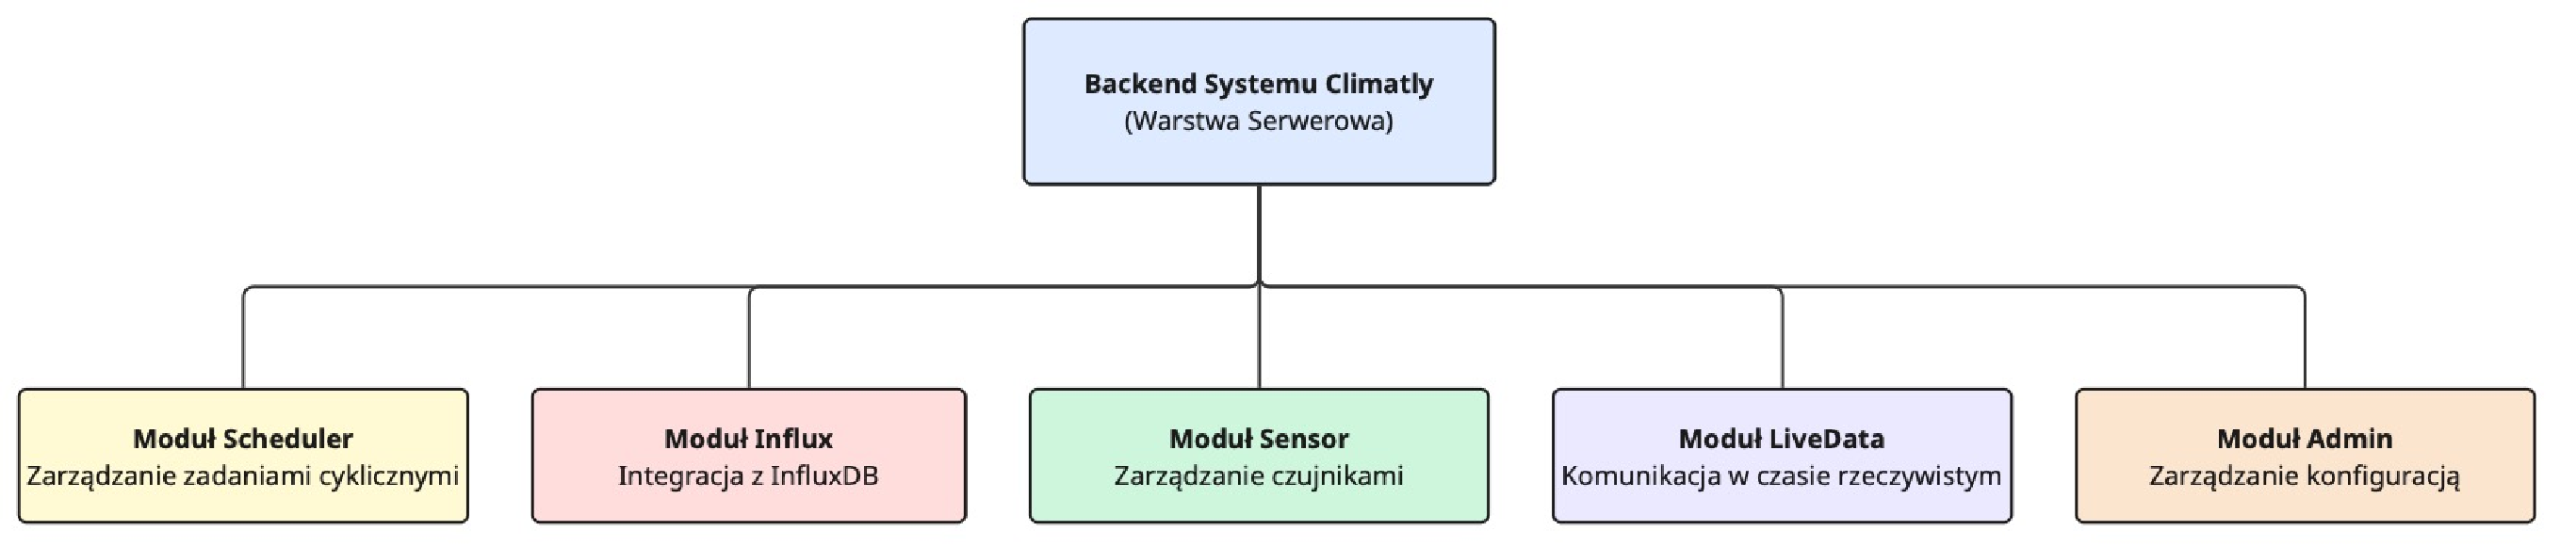
\includegraphics[width=1\textwidth]{Climatly-modules.pdf}
    \caption{Schemat modułów warstwy serwerowej systemu Climatly}
    \label{fig:moduly---systemu}
\end{figure}

\chapter{Technologie i narzędzia wykorzystane w projekcie}

Wybór odpowiednich technologii stanowił fundamentalny element procesu projektowania każdego systemu informatycznego. Podejmując decyzje technologiczne, kierowałem się przede wszystkim trzema nadrzędnymi zasadami: efektywną współpracą komponentów, elastycznością architektury oraz stabilnością zastosowanych rozwiązań.
Dążyłem do stworzenia systemu, w którym poszczególne warstwy i moduły funkcjonują jako spójna całość, jednocześnie zachowując luźne powiązania między sobą. Ta cecha okazała się szczególnie cenna w kontekście ewolucji wymagań biznesowych --- umożliwiła mi elastyczne dostosowywanie pojedynczych elementów systemu bez naruszania jego ogólnej struktury. Zaprojektowana architektura modułowa pozwala na rozwijanie i modyfikację poszczególnych funkcjonalności niezależnie od siebie, co znacząco usprawnia proces rozbudowy systemu.
Świadomie wybrałem technologie o ugruntowanej pozycji na rynku i szerokiej dokumentacji, co zminimalizowało ryzyko wystąpienia problemów typowo technicznych. Dzięki temu mogłem skoncentrować wysiłki na dostarczaniu funkcjonalności biznesowych, zamiast poświęcać czas na rozwiązywanie niespodziewanych problemów infrastrukturalnych. Niniejszy rozdział przedstawia szczegółowe uzasadnienie wyboru poszczególnych komponentów technologicznych warstwy serwerowej systemu Climatly.

\section{Java jako język programowania dla aplikacji backendowych}

W nowoczesnej architekturze aplikacji, warstwa backendowa odpowiada za przetwarzanie danych, implementację logiki biznesowej oraz komunikację z bazami danych. Współcześnie, dominującym standardem implementacji interfejsów backendowych stał się REST API (Representational State Transfer), który wykorzystuje protokół HTTP do komunikacji między klientem a serwerem, zapewniając skalowalność i elastyczność systemów rozproszonych [1].

Jako język programowania warstwy backendowej wybrałem Javę, która dzięki swoim unikalnym właściwościom, stała się jednym z wiodących języków w obszarze tworzenia warstw serwerowych, szczególnie w sektorze aplikacji korporacyjnych. Według raportu State of Java in the Enterprise, aż 70\% organizacji buduje nowe aplikacje pełnostackowe w Javie [2]. Ta silna pozycja wynika z kilku kluczowych cech tego języka, które okazały się wyjątkowo przydatne w moim projekcie:

\subsection*{Obiektowość}

Java to w pełni obiektowy język programowania, którego fundamenty opierają się na czterech głównych filarach koncepcji obiektowych: abstrakcji, hermetyzacji, dziedziczeniu i polimorfizmie. Obiektowość w Javie nie jest jedynie dodatkiem do języka, ale jego integralną częścią, co pozwala na tworzenie bardziej modularnego, skalowalnego i łatwiejszego w utrzymaniu kodu GeeksforGeeks, 2023 GeeksforGeeks.
Abstrakcja pozwala na ukrycie wewnętrznej złożoności systemu, eksponując jedynie niezbędne detale. Hermetyzacja (enkapsulacja) umożliwia ochronę danych poprzez ich ukrycie wewnątrz klasy i udostępnianie jedynie za pomocą kontrolowanych metod dostępowych. Dziedziczenie wspomaga wielokrotne wykorzystanie kodu poprzez tworzenie hierarchii klas, gdzie klasy potomne dziedziczą cechy i zachowania klas nadrzędnych. Polimorfizm zaś pozwala na wykorzystanie jednego interfejsu do różnych implementacji, co znacząco zwiększa elastyczność systemu Raygun, 2023

\subsection*{Wieloplatformowość}

Jedną z najbardziej charakterystycznych cech Javy jest jej niezależność od platformy sprzętowej i systemowej. Zasada „write once, run anywhere" umożliwia uruchamianie tego samego kodu na różnych systemach operacyjnych bez konieczności rekompilacji~\cite{bib:guvi2023}. Jest to możliwe dzięki Wirtualnej Maszynie Javy (JVM), która zapewnia warstwę abstrakcji między kodem aplikacji a systemem operacyjnym. W środowiskach korporacyjnych, gdzie często występuje heterogeniczna infrastruktura, ta cecha pozwala na znaczące obniżenie kosztów wdrożenia i utrzymania aplikacji.

\subsection*{Wydajność i skalowalność}

Java oferuje zaawansowane mechanizmy do obsługi wielowątkowości i przetwarzania współbieżnego, co jest kluczowe dla wysokowydajnych aplikacji backendowych. Wprowadzone w Javie 21 wirtualne wątki umożliwiają efektywną obsługę tysięcy równoczesnych połączeń, co jest niezbędne w systemach REST API o dużym obciążeniu. Dodatkowo, zaawansowane mechanizmy optymalizacji w JVM zapewniają wysoką wydajność aplikacji przy zachowaniu wszystkich zalet języka wysokiego poziomu.

Istotnym elementem wydajności Javy jest automatyczne zarządzanie pamięcią, realizowane przez moduł zwany Garbage Collector (GC). W przeciwieństwie do innych języków programowania, jak C czy C++, programista Javy nie musi ręcznie alokować i zwalniać pamięci, co eliminuje wiele potencjalnych błędów związanych z wyciekami pamięci. Garbage Collector automatycznie identyfikuje obiekty, które nie są już używane i zwalnia zajmowaną przez nie pamięć, co zwiększa stabilność aplikacji działających przez długi czas.

Skalowalność aplikacji Java wynika również z możliwości efektywnego wykorzystania zasobów sprzętowych. JVM automatycznie dostosowuje się do dostępnej pamięci i liczby procesorów, co pozwala na optymalne działanie zarówno na małych urządzeniach, jak i na potężnych serwerach.

\subsection*{Dojrzałość}

Java istnieje na rynku od ponad 25 lat, co czyni ją jednym z najbardziej ugruntowanych języków programowania w sektorze przedsiębiorstw. Ta długa obecność przełożyła się na stabilny i dojrzały ekosystem, bogaty w narzędzia, biblioteki oraz sprawdzone praktyki programistyczne.

Jedną z kluczowych zalet Javy w kontekście jej dojrzałości jest jej kompatybilność wsteczna. Kod napisany w starszych wersjach języka działa bez modyfikacji w nowszych wersjach, co minimalizuje koszty migracji i pozwala na ochronę dotychczasowych inwestycji w oprogramowanie. Ta cecha ma szczególne znaczenie w projektach długoterminowych, gdzie stabilność platformy jest priorytetem.

Mimo wspomnianiej kompatybilności wstecznej, Oracle regularnie wydaje nowe wersje Javy, wprowadzając innowacyjne rozwiązania przy jednoczesnym zachowaniu stabilności. W obecnym modelu wydawniczym, niektóre wersje otrzymują status LTS (Long---Term Support), co gwarantuje im długoterminowe wsparcie techniczne i aktualizacje bezpieczeństwa. Wsparcie dla wersji LTS może trwać nawet ponad dekadę --- przykładowo Java 8 będzie wspierana do 2030 roku. Ta przewidywalność cyklu życia jest nieoceniona w środowiskach korporacyjnych, gdzie nagłe zmiany technologiczne mogą generować znaczące ryzyko operacyjne

\subsection*{Bogaty ekosystem narzędzi}

Jednym z największych atutów Javy jest jej rozbudowany ekosystem bibliotek i frameworków wspierających tworzenie aplikacji backendowych. Dla twórców REST API szczególne znaczenie mają frameworki takie jak Spring Boot, który dzięki podejściu „convention over configuration" radykalnie upraszcza proces tworzenia aplikacji, automatyzując wiele aspektów konfiguracji i dostarczając gotowe rozwiązania dla typowych problemów.

Java oferuje również uniwersalne interfejsy dostępu do baz danych (JDBC) oraz zaawansowane frameworki ORM (Object---Relational Mapping), które abstrakcyjnie traktują różne systemy bazodanowe, upraszczając operacje na danych i zwiększając przenośność aplikacji.

\vspace{0.5cm}

Te kluczowe cechy czynią Javę językiem doskonale dopasowanym do wymagań nowoczesnych aplikacji backendowych, szczególnie w standardzie REST API.


\section{Spring Boot jako główny framework projektu}

Spring Boot to framework dla języka Java, który znacząco upraszcza tworzenie aplikacji webowych i serwerowych. Eliminuje konieczność skomplikowanych konfiguracji poprzez dostarczanie gotowych rozwiązań dla najczęstszych scenariuszy programistycznych. W projekcie Climatly Spring Boot pełni rolę kręgosłupa technologicznego, integrując wszystkie komponenty systemu w spójną całość i umożliwiając szybkie tworzenie zaawansowanych aplikacji serwerowych.

Technologia ta ma ugruntowaną pozycję w świecie aplikacji korporacyjnych. Zgodnie z kompleksowym badaniem firmy Snyk — wiodącej platformy cyberbezpieczeństwa dla deweloperów — obejmującym ponad 2000 respondentów, dokładnie 60\% deweloperów wykorzystuje Spring Framework do tworzenia głównych aplikacji produkcyjnych~\cite{bib:snyk2020}. Ta dominacja w sektorze enterprise wynika z niezawodności, dojrzałości ekosystemu oraz silnego wsparcia społeczności, co czyni Spring Boot preferowanym wyborem dla aplikacji o krytycznym znaczeniu biznesowym.

\subsection*{REST API --- uproszczenie implementacji}

REST API (Representational State Transfer) to styl komunikacji między aplikacjami, który wykorzystuje protokół HTTP wraz z jego metodami (GET, POST, PUT, DELETE) do wykonywania operacji na zasobach reprezentowanych w standardowych formatach jak JSON. REST opiera się na bezstanowości, co oznacza, że każde żądanie zawiera wszystkie informacje niezbędne do jego przetworzenia, oraz na jednolitym interfejsie, który umożliwia intuicyjne zarządzanie zasobami poprzez URL-e.

Spring Boot dostarcza wszystkie niezbędne narzędzia do efektywnego tworzenia REST API, dramatycznie upraszczając ten proces w porównaniu do tradycyjnych rozwiązań. Framework automatycznie włącza zaawansowane mechanizmy serializacji i deserializacji JSON poprzez Jackson, zarządza nagłówkami HTTP, zapewnia odpowiednie kody odpowiedzi oraz integruje walidację danych wejściowych z wykorzystaniem Bean Validation.

Dzięki adnotacjom takim jak \texttt{@RestController}, \texttt{@GetMapping}, \texttt{@PostMapping} czy \texttt{@RequestMapping}, tworzenie endpointów REST staje się deklaratywne i wymaga minimalnej ilości kodu.

\subsection*{Architektura Model-View-Controller (MVC)}

Spring Boot implementuje wzorzec Model-View-Controller (MVC), który zapewnia jasną separację odpowiedzialności w aplikacji oraz przejrzystą strukturę kodu. W aplikacjach REST API, które nie posiadają tradycyjnej warstwy prezentacji, wzorzec MVC przyjmuje nieco zmodyfikowaną formę, gdzie kontroler odpowiada za obsługę żądań HTTP i zwracanie danych w formacie JSON, model reprezentuje strukturę przesyłanych danych, a logika biznesowa jest wydzielona do warstwy serwisów.

W kontekście warstwy serwerowej projektu Climatly kontroler SensorController pełni rolę punktu wejścia dla wszystkich żądań związanych z czujnikami, definiując endpointy API i zarządzając przepływem danych. Warstwa serwisu zawiera całą logikę biznesową związaną z przetwarzaniem danych czujników, walidacją oraz orchestracją operacji na repozytoriach. Model reprezentuje strukturę danych przesyłanych między warstwami - zarówno encje bazodanowe jak Sensor, jak i obiekty DTO (Data Transfer Object) jak SensorResponse, które są dedykowane do komunikacji z klientem.

\begin{lstfloat}[htbp]
\begin{lstlisting}[language=java]
@RestController
@RequestMapping("/api/sensor")
public class SensorController {

    private final ISensorService sensorService;

    @GetMapping("/{id}")
    public ResponseEntity<SensorResponse> getSensorById(@PathVariable Short id) {
        return ResponseEntity.ok(sensorService.getSensorById(id));
    }
}
\end{lstlisting}
\caption{Przykład kontrolera w architekturze MVC}
\label{lst:sensor-controller-mvc}
\end{lstfloat}

\subsection*{Convention over Configuration - uproszczenie konfiguracji}

Dependency Injection i Inversion of Control stanowią fundament modularnej architektury systemu Climatly, umożliwiając luźne powiązania między komponentami. Spring Boot automatycznie wstrzykuje zależności poprzez konstruktor, eliminując konieczność ręcznego tworzenia obiektów i zarządzania ich cyklem życia. Wzorzec ten znacząco ułatwia testowanie poprzez możliwość łatwego mockowania zależności oraz zwiększa czytelność kodu przez jasne definiowanie zależności w konstruktorze. Framework automatycznie zarządza całym cyklem życia obiektów - od ich utworzenia, przez wstrzyknięcie zależności, aż po prawidłowe zniszczenie przy zamykaniu aplikacji:

\begin{lstfloat}[htbp]
\begin{lstlisting}[language=java]
@Service
@RequiredArgsConstructor
public class SensorService implements ISensorService {
    private final SensorRepository sensorRepository;
    private final SensorDataRepository sensorDataRepository;
    private final SensorMapper sensorMapper;

}
\end{lstlisting}
\caption{Przykład Dependency Injection w Spring Boot}
\label{lst:dependency-injection}
\end{lstfloat}

\subsection*{Korzyści dla projektu Climatly}

W kontekście projektu Climatly wybór Spring Boot przyniósł konkretne korzyści, które bezpośrednio wpłynęły na sukces implementacji. Framework umożliwił eliminację boilerplate code i automatyczną konfigurację, pozwalając na skupienie się na logice biznesowej zamiast na skomplikowanych ustawieniach infrastrukturalnych. Naturalne wsparcie dla modularności poprzez component scanning i package-based organization idealnie wpisało się w założenia architektoniczne systemu. Wbudowane mechanizmy automatycznego zarządzania transakcjami, serializacji JSON, walidacji danych oraz obsługi wyjątków znacząco przyspieszyły rozwój aplikacji, a natywne wsparcie dla Server-Sent Events umożliwiło implementację komunikacji w czasie rzeczywistym bez dodatkowych zależności. Dodatkowo, automatyczne mechanizmy task scheduling pozwoliły na eleganckie rozwiązanie problemu cyklicznej aktualizacji czujników, a integracja z wieloma bazami danych ułatwiła pracę z PostgreSQL i InfluxDB jednocześnie.

\section{Wykorzystane systemy baz danych}
W projekcie Climatly zastosowałem dwa komplementarne systemy baz danych: PostgreSQL jako tradycyjną bazę relacyjną oraz InfluxDB jako specjalistyczną bazę szeregów czasowych. Wybór dwóch różnych systemów bazodanowych nie był przypadkowy – wynikał z analizy specyficznych wymagań projektu oraz charakteru przetwarzanych danych.
\subsection*{PostgreSQL --- relacyjna baza metadanych}
PostgreSQL to zaawansowany, otwartoźródłowy system zarządzania relacyjnymi bazami danych (RDBMS), który w projekcie Climatly pełni rolę głównego repozytorium metadanych czujników. Wybór PostgreSQL był podyktowany kilkoma kluczowymi czynnikami:

\begin{itemize}
  \item \textbf{Integralność danych} --- PostgreSQL oferuje pełne wsparcie dla ACID (Atomicity, Consistency, Isolation, Durability), co zapewnia spójność danych nawet w przypadku awarii systemu. Jest to krytyczne dla danych kontekstowych, takich jak lokalizacje czujników czy ich statusy operacyjne.
  \item \textbf{Złożone relacje} --- Model relacyjny doskonale sprawdza się przy modelowaniu złożonych zależności między obiektami biznesowymi. W projekcie Climatly pozwoliło to na efektywne reprezentowanie powiązań między czujnikami, lokalizacjami, budynkami i piętrami.
  \item \textbf{Zaawansowane zapytania} --- PostgreSQL oferuje rozbudowany język SQL, który umożliwia tworzenie złożonych zapytań analitycznych oraz filtrowanie i agregację danych według wielu kryteriów.
\end{itemize}

\subsection*{InfluxDB --- nierelacyjna baza szeregów czasowych}
InfluxDB to wyspecjalizowana, nierelacyjna baza danych zaprojektowana do efektywnego przechowywania i analizy danych szeregów czasowych. W projekcie Climatly pełni ona rolę repozytorium przechowującego surowe odczyty z czujników. Wykorzystanie InfluxDB było zdeterminowane następującymi czynnikami:

\begin{itemize}
  \item \textbf{Optymalizacja pod kątem szeregów czasowych} --- InfluxDB jest zoptymalizowana pod kątem przechowywania i przetwarzania dużych wolumenów danych uporządkowanych chronologicznie, co idealnie odpowiada charakterowi odczytów z czujników meteorologicznych.
  \item \textbf{Wysoka wydajność zapisu} --- System oferuje znacząco wyższą przepustowość zapisu w porównaniu do tradycyjnych baz relacyjnych, co jest kluczowe przy ciągłym strumieniowaniu danych z sieci czujników.
  \item \textbf{Efektywne zapytania czasowe} --- InfluxDB udostępnia język zapytań Flux, który umożliwia wydajne wykonywanie operacji na zakresach czasowych, co jest fundamentalnym wymaganiem dla analizy trendów pogodowych.
\end{itemize}

\subsection*{Podział odpowiedzialności między bazami danych}
W architekturze systemu Climatly przyjąłem jasny podział odpowiedzialności między obydwiema bazami danych:

\textbf{PostgreSQL przechowuje:}
\begin{itemize}[noitemsep,topsep=0pt]
\item Metadane czujników (lokalizacja, nazwa, piętro, budynek)
\item Statusy operacyjne urządzeń (online, offline, błąd)
\item Konfigurację systemu (częstotliwość odświeżania danych)
\item Rejestry awarii i zdarzeń systemowych
\item Najnowsze agregacje danych do szybkiego dostępu
\end{itemize}
\vspace{10pt}
\textbf{InfluxDB przechowuje:}
\begin{itemize}[noitemsep,topsep=0pt]
\item Surowe odczyty z czujników (temperatura, wilgotność, ciśnienie)
\item Pełne szeregi czasowe wszystkich pomiarów
\item Historyczne dane z precyzyjnymi znacznikami czasowymi
\end{itemize}

\section{Integracja baz danych w modelu ORM}

Komunikacja z bazą PostgreSQL w warstwie backendowej odbywa się z wykorzystaniem Spring Data JPA, która implementuje koncepcję ORM (Object-Relational Mapping). ORM to paradygmat programistyczny, który umożliwia mapowanie obiektów języka Java bezpośrednio na struktury relacyjne bazy danych. W praktyce oznacza to, że klasy Javy z odpowiednimi adnotacjami stają się reprezentacją tabel w bazie danych, a ich instancje odzwierciedlają poszczególne rekordy.

Dzięki zastosowaniu ORM w projekcie Climatly:
\begin{itemize}[noitemsep,topsep=2pt]
\item Nie ma potrzeby pisania ręcznych zapytań SQL - framework generuje je automatycznie na podstawie nazw metod w repozytoriach
\item Encje Javy (np. \texttt{Sensor}, \texttt{Location}) są bezpośrednio przekształcane w tabele bazodanowe
\item Relacje między obiektami (jak one-to-many czy many-to-many) są wyrażane za pomocą adnotacji takich jak \texttt{@OneToMany} czy \texttt{@ManyToMany}
\item Operacje CRUD stają się proste i intuicyjne - wystarczy wywołać metody na obiektach repozytoriów
\end{itemize}

Kluczowe elementy tej integracji to:
\begin{itemize}[noitemsep,topsep=2pt]
\item \textbf{Repozytoria Spring Data} - interfejsy, które automatycznie implementują podstawowe operacje CRUD na encjach, znacząco redukując ilość kodu boilerplate.
\item \textbf{Adnotacje JPA} - deklaratywne definicje mapowań obiektowo-relacyjnych, które upraszczają transformację między światem obiektowym Javy a relacyjnym modelem bazy danych.
\end{itemize}


\section{Dodatkowe narzędzia i biblioteki}

W projekcie Climatly, oprócz podstawowych technologii takich jak Java, Spring Boot i systemy bazodanowe, zastosowałem szereg specjalistycznych narzędzi, które usprawniły codzienną pracę nad kodem i przyspieszyły rozwój aplikacji. Wykorzystanie tych narzędzi znacząco zoptymalizowało wiele procesów twórczych, takich jak migracje bazy danych, zarządzanie powtarzalnym kodem, konfigurowanie lokalnych środowisk programistycznych czy monitorowanie działania systemu poprzez logowanie.

\subsection*{Docker --- konteneryzacja aplikacji}

Rola Dockera w nowoczesnym procesie wytwarzania oprogramowania jest niezastąpiona. Docker to platforma umożliwiająca tworzenie, wdrażanie i uruchamianie aplikacji w kontenerach, które zawierają wszystkie niezbędne zależności i biblioteki potrzebne do działania aplikacji. Kontenery te są lekkie, przenośne i izolowane od systemu operacyjnego, co umożliwia spójne działanie aplikacji niezależnie od środowiska.

W pracy developerskiej wykorzystałem Docker Compose, który doskonale integruje się ze Spring Bootem i umożliwia szybkie przygotowanie lokalnego środowiska deweloperskiego. Docker Compose pozwolił mi na tworzenie i zarządzanie wieloma kontenerami jednocześnie, definiując całą infrastrukturę jako kod. Dzięki temu mogłem zdefiniować zarówno bazę PostgreSQL, jak i InfluxDB w jednym pliku konfiguracyjnym:

\begin{lstfloat}[htbp]
\begin{lstlisting}[language=yaml]
version: '3.8'
services:
  postgres-db-local:
    image: 'postgres:latest'
    container_name: postgres-db
    environment:
      - POSTGRES_DB=mydatabase
      - POSTGRES_USER=kamil.golawski
      - POSTGRES_PASSWORD=secret
    ports:
      - '5432:5432'
    volumes:
      - pgdata:/var/lib/postgresql/data
      - ./init.sql:/docker-entrypoint-initdb.d/init.sql
    restart: unless-stopped

  influxdb:
    image: influxdb:2.7
    container_name: influxdb
    ports:
      - "8086:8086"
    volumes:
      - ./influxdb_data:/var/lib/influxdb2
    environment:
      - DOCKER_INFLUXDB_INIT_MODE=setup
      - DOCKER_INFLUXDB_INIT_USERNAME=admin
      - DOCKER_INFLUXDB_INIT_PASSWORD=adminadmin
      - DOCKER_INFLUXDB_INIT_ORG=SKNI
      - DOCKER_INFLUXDB_INIT_BUCKET=czujniki
    restart: unless-stopped
\end{lstlisting}
\caption{Fragment pliku \texttt{docker-compose.yaml} definiującego lokalne środowisko developerskie}
\label{lst:docker-compose}
\end{lstfloat}

Kluczową zaletą tego rozwiązania jest możliwość przechowywania danych bez ingerencji w środowisko produkcyjne, co pozwoliło mi na swobodne eksperymentowanie, testowanie zmian i rozwijanie funkcjonalności bez ryzyka uszkodzenia danych produkcyjnych.

Najważniejszym elementem konteneryzacji dla środowiska produkcyjnego jest Dockerfile, który definiuje wszystkie procesy niezbędne do uruchomienia aplikacji na docelowej infrastrukturze, niezależnie czy będzie to Kubernetes (K8s), czy AWS Elastic Container Service (ECS) w razie potrzeby przeniesienie backendu na zupełnie nową infrastrukturę. Ten Dockerfile automatyzuje proces budowania i wdrażania aplikacji, co znacząco upraszcza konfigurację środowiska produkcyjnego i minimalizuje ryzyko błędów związanych z różnicami między środowiskami.


\clearpage

\subsection*{Liquibase - zarządzanie zmianami schematu bazy danych}

Liquibase to narzędzie open-source przeznaczone do zarządzania i wersjonowania zmian w schemacie bazy danych. W projekcie Climatly odgrywa ono kluczową rolę w utrzymaniu spójności struktury bazy danych PostgreSQL na różnych środowiskach.

Omawiane narzędzie używa koncepcji ``changesetów'' - atomowych, ponumerowanych zestawów zmian, które są sekwencyjnie aplikowane do bazy danych. Każdy changeset jest identyfikowany przez unikalne ID oraz autora, co zapewnia pełną kontrolę nad historią zmian i możliwość śledzenia, kto i kiedy wprowadził konkretne modyfikacje. Z początku projektu Liquibase został przeze mnie wykorzystany do zdefiniowania początkowego schematu tabel, który bardziej szczegółowo będzie omówiony w rozdziale 3.

\begin{lstfloat}[htbp]
\begin{lstlisting}[language=xml]
<changeSet id="1736355579438-3" author="kamilgolawski">
    <createTable tableName="sensor">
        <column autoIncrement="true" name="id" type="SMALLINT">
            <constraints nullable="false" primaryKey="true" primaryKeyName="pk_sensor"/>
        </column>
        <column name="status" type="VARCHAR(255)"/>
        <column name="last_update" type="DATETIME"/>
        <column name="temperature" type="SMALLINT"/>
        <column name="humidity" type="INT"/>
        <column name="pressure" type="INT"/>
        <column name="location_id" type="SMALLINT"/>
    </createTable>
</changeSet>
\end{lstlisting}
\caption{Fragment pliku inicjalizującego schemat bazy danych}
\label{lst:liquibase-init}
\end{lstfloat}

W miarę ewolucji aplikacji, pojawiały się potrzeby modyfikacji struktury bazy danych. Zamiast ręcznego wykonywania skryptów SQL na każdym środowisku, Liquibase umożliwił mi deklaratywne definiowanie zmian, które następnie były automatycznie aplikowane podczas startu aplikacji, jednocześnie dbając o spójność wcześniejszych changesetów oraz obecnych już realnych danych w tabeli, na których stratę nie mogłem sobie pozwolić.

\begin{lstfloat}[htbp]
\begin{lstlisting}[language=xml]
<changeSet id="1739223645331-1" author="kamilgolawski">
    <addColumn tableName="location">
        <column name="faculty_abbreviation" type="VARCHAR(10)"/>
    </addColumn>
</changeSet>

<changeSet id="drop_gas_resistance_columns" author="kamilgolawski">
    <dropColumn tableName="sensor_data">
        <column name="gas_resistance"/>
    </dropColumn>
</changeSet>
\end{lstlisting}
\caption{Przykład modyfikacji struktury bazy danych}
\label{lst:liquibase-modify}
\end{lstfloat}

\vspace{2cm}

\subsection*{Lombok - generowanie schematycznego kodu}

Lombok to popularna biblioteka Javy, która znacząco usprawnia proces programowania poprzez redukcję powtarzalnego kodu. Java jako język jest często krytykowana za wymaganie dużej ilości tzw. boilerplate code - standardowego, powtarzalnego kodu, który programista musi pisać w wielu miejscach. Dotyczy to szczególnie klas przechowujących dane, gdzie dla każdego pola trzeba często tworzyć gettery, settery, konstruktory, metody equals, hashCode i toString.

Wykorzystanie Lomboka szczególnie usprawnia pracę ze Springiem, który dla optymalnego działania wymaga specyficznych konstruktorów i metod dostępowych. To, co normalnie wymagałoby napisania dziesiątek linii kodu, z Lombokiem sprowadza się do dodania jednej adnotacji co dramatycznie zwiększa czytelność i zmniejsza ilość kodu, który musi być utrzymywany.

\begin{lstfloat}[htbp]
\begin{lstlisting}[language=java]
@Builder
@NoArgsConstructor
@AllArgsConstructor
@ToString
@Getter
@Setter
@Entity
@Table(name = "sensor_data")
public class SensorData {

  @Id
  @GeneratedValue(strategy = GenerationType.IDENTITY)
  @Column(name = "data_id")
  private Long dataId;

  @ManyToOne(fetch = FetchType.EAGER)
  @JoinColumn(name = "sensor_id", nullable = false)
  private Sensor sensor;

  private ZonedDateTime timestamp;

  @Column(precision = 5, scale = 1)
  private BigDecimal temperature;

  private Integer humidity;

  private Integer pressure;
}
\end{lstlisting}
\caption{Fragment klasy encji Sensor z adnotacjami Lombok}
\label{lst:lombok}
\end{lstfloat}
\vfill

\vspace{2cm}

\subsection*{Profile Spring Boot - zarządzanie konfiguracją}

Profile Spring Boot to mechanizm umożliwiający elastyczne dostosowanie konfiguracji aplikacji w zależności od środowiska uruchomieniowego. W projekcie Climatly wykorzystałem profile do oddzielenia konfiguracji środowiska developerskiego od produkcyjnego poprzez zdefiniowanie różnych parametrów połączenia do bazy danych oraz konfigurację poziomów logowania. W środowisku developerskim zastosowałem bardziej szczegółowy poziom logowania, co znacząco ułatwia debugowanie i śledzenie przepływu danych, podczas gdy w środowisku produkcyjnym ograniczyłem logi do najważniejszych komunikatów, co optymalizuje wydajność aplikacji. Oczekiwany profil aktywuje się jako parametr przy uruchamianiu aplikacji z pliku wykonywalnego JAR.

\begin{lstfloat}[H]
\begin{lstlisting}[language=yaml]
# application-local.yaml
spring:
  datasource:
    url: ${DB_URL}
  mvc:
    async:
      request-timeout: 360000
logging:
  level:
    root: INFO
    skni.kamilG: DEBUG
\end{lstlisting}
\caption{Fragment konfiguracji dla profilu lokalnego}
\label{lst:profile-local}
\end{lstfloat}

\subsection*{Swagger --- automatyczna dokumentacja API}

Swagger to narzędzie do automatycznego generowania dokumentacji interfejsu API w formacie OpenAPI. W projekcie Climatly zastosowałem integrację ze Swagger, co pozwala nie tylko na łatwą integrację aplikacji klienckiej z backendem, lecz również otwiera furtkę dla zewnętrznych klientów, jasno definiując jakie są dostępne endpointy, jakie są ich wymagania wejściowe oraz oczekiwane formaty odpowiedzi. Dzięki tej dokumentacji, deweloperzy frontendowi otrzymują precyzyjny opis wszystkich dostępnych funkcji API bez konieczności ręcznego tworzenia dokumentacji, która mogłaby się szybko zdezaktualizować.

\begin{figure}[H]
    \centering
    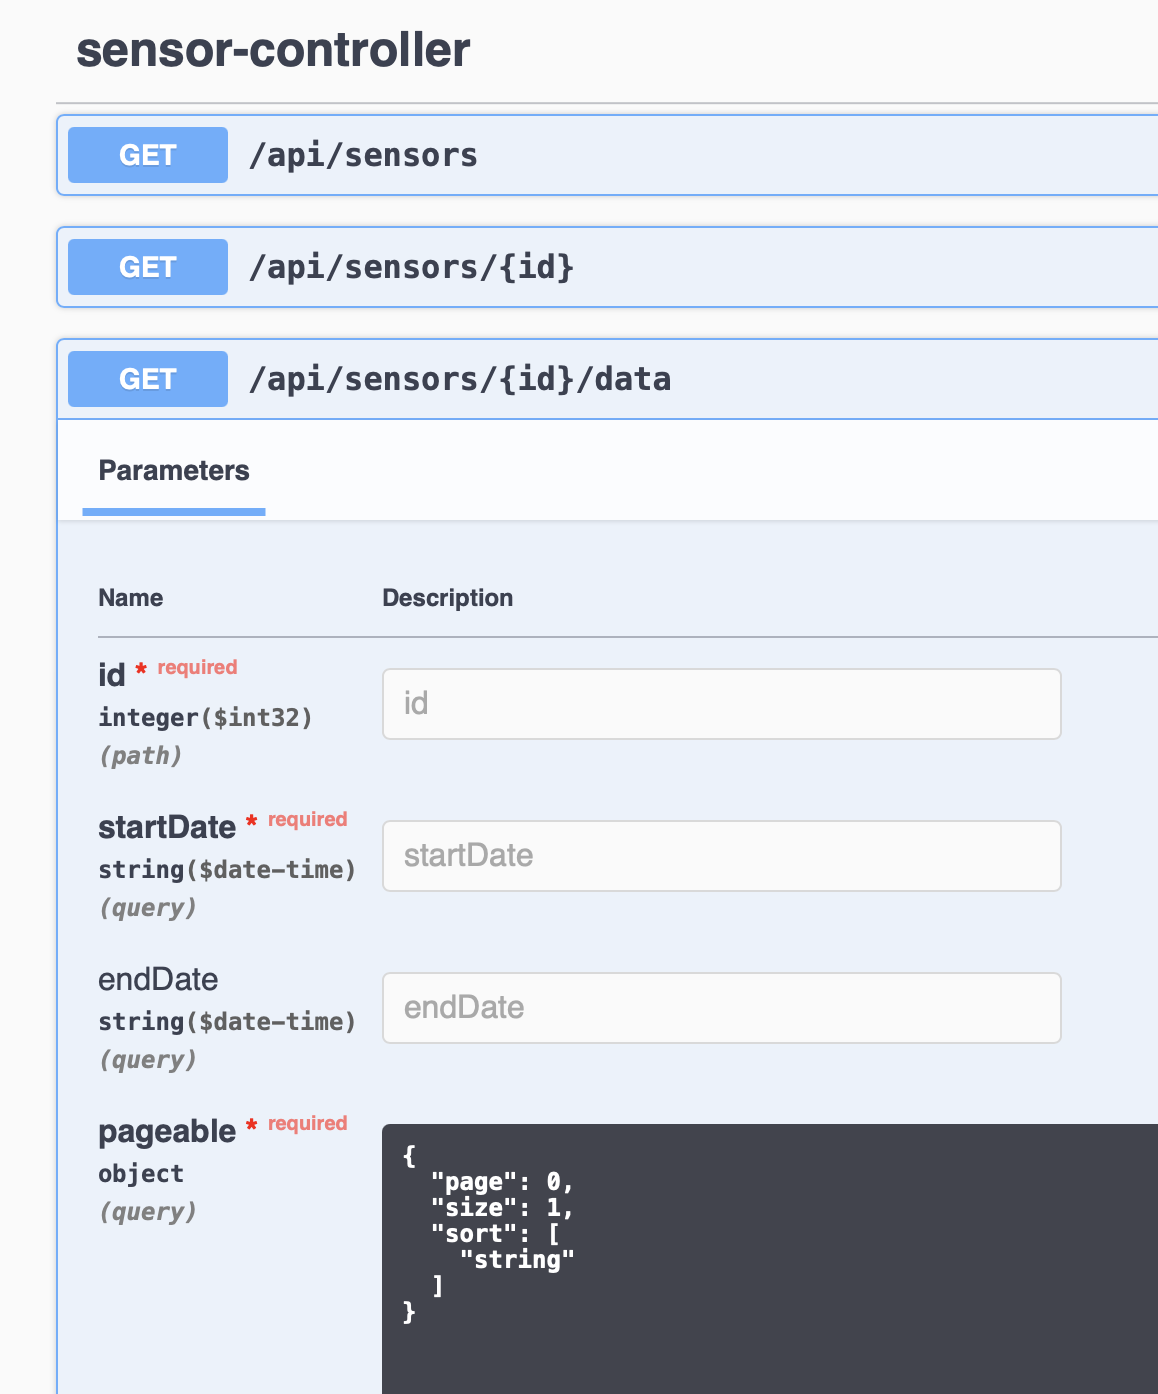
\includegraphics[width=0.9\textwidth]{swagger.png}
    \caption{Przykładowy widok dokumentacji API wygenerowanej przez Swagger UI}
    \label{fig:swagger-ui}
\end{figure}

\chapter{Modularność oraz szczegółowa architektura systemu}

Projektując warstwę serwerową systemu Climatly, przyjąłem architekturę modularną, która wynika bezpośrednio z wcześniej zidentyfikowanych funkcjonalności oraz założeń projektowych. Modularność nie była jedynie wyborem architektonicznym, ale koniecznością wynikającą z różnorodności wymagań technicznych oraz potrzeby zachowania elastyczności systemu, aby potencjalne awarie jednego z modułów z góry nie skreślały działania pozostałych części.

Architektura modularna przynosi kilka istotnych korzyści w kontekście systemu zarządzania danymi pogodowymi. Po pierwsze, umożliwia separację odpowiedzialności — każdy moduł koncentruje się na konkretnym aspekcie działania systemu, co ułatwia zrozumienie kodu i jego utrzymanie. Po drugie, wspiera niezależny rozwój — różne funkcjonalności mogą być rozwijane równolegle bez ryzyka konfliktów. Po trzecie, zwiększa testowalność — każdy moduł może być testowany w izolacji, co upraszcza proces weryfikacji poprawności działania. Wreszcie, ułatwia diagnozowanie problemów — błędy są lokalizowane w obrębie konkretnych modułów, co przyspiesza proces debugowania.

\begin{itemize}[itemsep=3pt,topsep=5pt,parsep=0pt]
\item \textbf{Separacja odpowiedzialności} --- Każdy moduł koncentruje się na konkretnym aspekcie działania systemu, co ułatwia zrozumienie kodu i jego utrzymanie. Programista pracujący nad modułem Scheduler nie musi znać szczegółów implementacji komunikacji z InfluxDB.

\item \textbf{Niezależny rozwój} --- Różne funkcjonalności mogą być rozwijane równolegle bez ryzyka konfliktów. Podczas gdy jeden developer optymalizuje zapytania Flux, inny może skupić się na ulepszaniu mechanizmów SSE.

\item \textbf{Zwiększona testowalność} --- Każdy moduł może być testowany w izolacji, co upraszcza proces weryfikacji poprawności działania. Testy modułu Admin nie wymagają uruchomienia bazy InfluxDB.

\item \textbf{Łatwiejsze diagnozowanie problemów} --- Błędy są lokalizowane w obrębie konkretnych modułów, co przyspiesza proces debugowania. Problemy z połączeniami SSE nie wpływają na pobieranie danych historycznych.

\item \textbf{Elastyczność w rozbudowie} --- Nowe funkcjonalności można dodawać jako osobne moduły bez modyfikacji istniejącego kodu, zachowując stabilność działającego systemu.
\end{itemize}

\section{Podział odpowiedzialności w systemie}

\subsection{Moduł Sensor --- zarządzanie czujnikami}
Moduł Sensor stanowi rdzeń systemu Climatly i odpowiada za kompleksowe zarządzanie danymi czujników meteorologicznych. Jest to najbardziej rozbudowany moduł, który integruje dane z dwóch źródeł: metadane z bazy PostgreSQL oraz surowe odczyty z bazy InfluxDB lecz nie odpowiada za ich bezpośredni odczyt.

\textbf{Główne zadania modułu:}
\begin{itemize}[itemsep=2pt,topsep=4pt,parsep=0pt]
\item \textbf{Zarządzanie metadanymi czujników} --- Moduł przechowuje i zarządza informacjami kontekstowymi o czujnikach, takimi jak lokalizacja geograficzna, przypisanie do konkretnego budynku i piętra, status operacyjny oraz konfigurację częstotliwości odświeżania danych. Te metadane są kluczowe dla nadania sensu surowym odczytom pomiarowym.

\item \textbf{Udostępnianie danych historycznych} --- Realizuje interfejs REST API umożliwiający pobieranie historycznych danych pomiarowych w różnych przekrojach czasowych i przestrzennych. Obsługuje filtrowanie według dat, lokalizacji oraz konkretnych czujników, zapewniając paginację dla dużych zestawów danych.

\item \textbf{Agregacja i kontekstualizacja danych} --- Łączy oraz agreguje surowe odczyty z InfluxDB z metadanymi z PostgreSQL, tworząc kompletne odpowiedzi zawierające zarówno wartości pomiarowe, jak i informacje o lokalizacji oraz statusie czujników.
\end{itemize}


Serce modułu stanowi encja \texttt{Sensor}, która reprezentuje fizyczny czujnik meteorologiczny w systemie. Encja ta łączy w sobie zarówno aktualne odczyty pomiarowe, jak i metadane opisujące czujnik:

\begin{lstfloat}[H]
\begin{lstlisting}[language=java]
@Entity
@Table(name = "sensor")
public class Sensor implements Serializable{
    @Id
    @GeneratedValue(strategy = GenerationType.IDENTITY)
    private Short id;

    @Enumerated(EnumType.STRING)
    private SensorStatus status;

    private ZonedDateTime lastUpdate;
    private BigDecimal temperature;
    private Integer humidity;
    private Integer pressure;
    private Short refreshRate;
    private Short floor;

    @OneToOne(cascade = CascadeType.ALL)
    @JoinColumn(name = "location_id")
    private Location location;


    public void updateFromSensorData(SensorData latestSensorData, Clock clock) {
        this.temperature = latestSensorData.getTemperature();
        this.humidity = latestSensorData.getHumidity();
        this.pressure = latestSensorData.getPressure();
        this.lastUpdate = ZonedDateTime.now(clock);
    }
}
\end{lstlisting}
\caption{Encja Sensor --- centralna klasa modułu}
\label{lst:sensor-entity}
\end{lstfloat}


\subsection{Moduł Influx --- integracja z bazą szeregów czasowych}

Moduł Influx stanowi wyspecjalizowany komponent systemu dedykowany wyłącznie odczytom danych z czujników meteorologicznych. Jest jedynym modułem posiadającym bezpośrednie połączenie z bazą szeregów czasowych InfluxDB, co zapewnia kontrolowaną i scentralizowaną komunikację z tym krytycznym źródłem danych. Wydzielenie funkcjonalności do osobnego modułu skutecznie rozwiązało wyzwania związane ze złożonym wykorzystywaniem języka Flux do konstruowania zapytań czasowych.

\vspace{0.5em}
\textbf{Główne odpowiedzialności modułu:}
\begin{itemize}[itemsep=2pt,topsep=4pt,parsep=0pt]
\item \textbf{Wyłączny dostęp do InfluxDB} --- Stanowi jedyną bramę komunikacyjną z bazą szeregów czasowych, centralizując wszystkie operacje pobierania danych pomiarowych i eliminując duplikację połączeń w systemie.

\item \textbf{Walidacja i mapowanie danych} --- Sprawdza poprawność i kompletność pobranych odczytów, obsługuje sytuacje z brakującymi lub opóźnionymi danymi. Po poprawnej walidacji przekształca surowe odpowiedzi InfluxDB na typowane obiekty Java wykorzystywane w pozostałych częściach systemu.

\item \textbf{Dynamiczne generowanie zapytań Flux} --- Automatycznie konstruuje zoptymalizowane zapytania w języku Flux na podstawie zewnętrznych parametrów, takich jak identyfikator czujnika czy częstotliwość odświeżania danych. Dzięki temu inne moduły nie muszą wchodzić w bezpośrednią interakcję ze złożoną składnią Flux.

\end{itemize}

\vspace{-0.4em}

Kluczowym elementem modułu jest metoda \texttt{buildQueryWithParams()}, która dynamicznie konstruuje zapytania w języku Flux dostosowane do specyficznych wymagań każdego żądania:

\begin{lstfloat}[H]
\begin{lstlisting}[language=java]
private String buildQueryWithParams(Short sensorId, Short refreshRate) {
    return String.format(
        """
        from(bucket: "%s")
          |> range(start: -%ds)
          |> filter(fn: (r) => r["_measurement"] == "sensor_readings")
          |> filter(fn: (r) => r["_field"] == "%s" or
                               r["_field"] == "%s" or
                               r["_field"] == "%s" or
                               r["_field"] == "%s")
          |> pivot(rowKey:["_time"], columnKey: ["_field"], valueColumn: "_value")
          |> filter(fn: (r) => r["sensor_id"] == %s)
          |> last(column: "_time")
        """,
        bucket,
        refreshRate,
        HUMIDITY_FIELD,
        PRESSURE_FIELD,
        TEMPERATURE_FIELD,
        SENSOR_ID_FIELD,
        sensorId);
}
\end{lstlisting}
\caption{Metoda generująca zapytania Flux w module Influx}
\label{lst:flux-query}
\end{lstfloat}

\subsection{Moduł LiveData --- komunikacja w czasie rzeczywistym}

Moduł LiveData implementuje zaawansowaną funkcjonalność strumieniowania danych w czasie rzeczywistym przy użyciu technologii Server-Sent Events (SSE). Stanowi kluczowy komponent umożliwiający aplikacji klienckiej otrzymywanie aktualnych odczytów z czujników w czasie rzeczywistym bez obciążania serwera.

\textbf{Główne odpowiedzialności modułu:}
\begin{itemize}[itemsep=2pt,topsep=0pt,parsep=0pt]
\vspace{0.5em}
\item \textbf{Zarządzanie połączeniami SSE} --- Utrzymuje aktywne połączenia z klientami, zarządza ich cyklem życia oraz automatycznie usuwa nieaktywne połączenia w przypadku przerwania transmisji lub timeout-u.

\item \textbf{Subskrypcje tematyczne} --- Umożliwia klientom subskrybowanie konkretnych czujników lub wszystkich aktualizacji w systemie, efektywnie filtrując i kierując odpowiednie powiadomienia do zainteresowanych odbiorców.

\item \textbf{Rozgłaszanie aktualizacji} --- Natychmiast wysyła powiadomienia o nowych odczytach do wszystkich zainteresowanych klientów, zapewniając synchronizację danych w czasie rzeczywistym.

\item \textbf{Optymalizacja przepustowości} --- Implementuje mechanizmy heartbeat, reconnection oraz buforowania zdarzeń, minimalizując obciążenie sieci przy jednoczesnym zachowaniu niezawodności połączeń.
\end{itemize}

Kluczowym elementem modułu jest kontroler \texttt{LiveController}, który demonstruje zaawansowaną obsługę połączeń Server-Sent Events z precyzyjną konfiguracją nagłówków HTTP:

\begin{lstfloat}[H]
\begin{lstlisting}[language=java]
@RestController
@RequestMapping("/live-api/sensors")
public class LiveController {

    private final ISseEmitterService sseEmitterService;

    @GetMapping(produces = MediaType.TEXT_EVENT_STREAM_VALUE)
    public ResponseEntity<SseEmitter> streamAllSensorsUpdates(
        @RequestHeader(value = "Last-Event-ID", required = false) String lastEventId,
        HttpServletResponse response) {

        String clientId = UUID.randomUUID().toString();
        SseEmitter emitter = sseEmitterService.createSseEmitter(clientId, null);
        return ResponseEntity.ok().contentType(MediaType.TEXT_EVENT_STREAM).body(emitter);
    }
\end{lstlisting}
\caption{Fragment kontrolera SSE obsługujący strumieniowanie wszystkich czujników}
\label{lst:live-controller}
\end{lstfloat}


\subsection{Moduł Scheduler --- automatyzacja zadań}

Moduł Scheduler stanowi prosty choć zaawansowany komponent systemu, który powstał z konieczności implementacji indywidualnego procesowania każdego czujnikia. Wcześniejsze podejście generowało istotne problemy operacyjne, które szczegółowo omówię w rozdziale 4. Moduł odpowiada za efektywne zarządzanie pulą wirtualnych wątków, przydzielając każdemu z nich niezależne zadania cyklicznej aktualizacji danych pomiarowych.

Główną odpowiedzialością modułu jest koordynacja harmonogramu pobierania najnowszych odczytów z bazy InfluxDB oraz synchronizacja metadanych w bazie PostgreSQL dla każdego czujnika zgodnie z jego indywidualnie skonfigurowanymi parametrami częstotliwości. Rozwiązanie oparte na mapie zadań umożliwia dynamiczne dodawanie, usuwanie oraz modyfikowanie harmonogramów poszczególnych czujników bez destabilizacji pozostałych elementów systemu.

Dodatkowo, moduł implementuje mechanizm automatycznego wykrywania nieaktywnych czujników oraz oznaczania ich statusu jako błędnego, co zapewnia kompleksowe monitorowanie stanu całej infrastruktury pomiarowej.

Centralnym elementem modułu jest klasa \texttt{Scheduler}, która funkcjonuje jako koordynator wszystkich zadań cyklicznych w systemie:


\vspace{1em}
\begin{lstlisting}[language=java]
@Service
public class Scheduler {

   private final Map<Short, ScheduledFuture<?>> scheduledTasks = new ConcurrentHashMap<>();
   private final SensorUpdateService sensorUpdateService;
   private final TaskScheduler taskScheduler;

   @Value("${scheduler.default-rate:180}")
   private short defaultRate;

   @PostConstruct
   public void init() {
       startDefaultTasks();
   }

   public void updateTaskRates(List<Sensor> sensorsToUpdate) {
       sensorsToUpdate.forEach(sensor -> {
           ScheduledFuture<?> existingTask = scheduledTasks.get(sensor.getId());
           if (existingTask != null) {
               existingTask.cancel(false);
               log.debug("Cancelled existing task for sensor {}", sensor.getId());
           }

           short rate = Optional.ofNullable(sensor.getRefreshRate()).orElse(defaultRate);
           ScheduledFuture<?> newTask = taskScheduler.scheduleAtFixedRate(
               () -> updateSingleSensor(sensor),
               Duration.ofSeconds(rate)
           );
           scheduledTasks.put(sensor.getId(), newTask);
           log.debug("Scheduled task for sensor {} with rate {} seconds", sensor.getId(), rate);
       });
   }

   private void updateSingleSensor(Sensor sensor) {
       try {
           sensorUpdateService.updateSingleSensor(sensor);
       } catch (Exception e) {
           log.error("Failed to update sensor {}: {}", sensor.getId(), e.getMessage());
       }
   }

   @PreDestroy
   public void shutdown() {
       scheduledTasks.values().forEach(task -> task.cancel(false));
       scheduledTasks.clear();
       log.info("Cleaned up all scheduled tasks");
   }
}
\end{lstlisting}
\caption{Klasa Scheduler zarządzająca harmonogramem zadań cyklicznych}
\label{lst:scheduler}

\subsection{Moduł Admin --- zarządzanie konfiguracją}

Moduł Admin stanowi wyspecjalizowany komponent odpowiedzialny za zdalne zarządzanie konfiguracją systemu oraz parametrami operacyjnymi czujników. Jest to moduł o ograniczonym dostępie, zabezpieczony mechanizmem autoryzacji opartym na kluczu API, który umożliwia administratorom wprowadzanie zmian w czasie rzeczywistym bez konieczności fizycznej ingerencji w infrastrukturę. Główną charakterystyką modułu jest implementacja operacji wsadowych, które pozwalają na jednoczesną modyfikację wielu czujników, co znacząco usprawnia administrację rozległą siecią urządzeń pomiarowych.

Moduł oferuje dwie kluczowe funkcjonalności: zarządzanie statusem czujników poprzez aktywację, dezaktywację lub oznaczanie jako niesprawnych oraz konfigurację częstotliwości odświeżania danych dla poszczególnych urządzeń. Operacje wsadowe umożliwiają administratorom efektywne zarządzanie całymi grupami czujników jednocześnie, co jest szczególnie istotne w przypadku konieczności szybkich zmian konfiguracyjnych na dużą skalę. Dodatkowo, moduł automatycznie propaguje zmiany do modułu Scheduler, zapewniając natychmiastowe odzwierciedlenie nowych ustawień w harmonogramie zadań systemowych.

Centralnym elementem modułu jest serwis \texttt{AdminService}, który implementuje generyczną metodę obsługującą różne typy poleceń administracyjnych:

\begin{lstlisting}[language=java,caption={Serwis Admin z metodą aktualizacji wsadowej},label={lst:admin-service}]
@Service
public class AdminService implements IAdminService {

   private final SensorRepository sensorRepository;
   private final Scheduler scheduler;

   @Transactional
   public <T extends SensorCommand> void updateSensors(List<T> commands) {
       List<Sensor> sensorsToUpdate = commands.stream()
           .map(command -> sensorRepository.findById(command.sensorId())
               .map(sensor -> {
                   if (command instanceof RefreshRateCommand refreshRateCommand) {
                       sensor.setRefreshRate(refreshRateCommand.refreshRate());
                       log.info("Updating sensor {} refresh rate to {} seconds",
                           sensor.getId(), refreshRateCommand.refreshRate());
                   } else if (command instanceof StatusCommand statusCommand) {
                       sensor.setStatus(statusCommand.status());
                       log.info("Updating sensor {} status to {}",
                           sensor.getId(), statusCommand.status());
                   }
                   return sensor;
               })
               .orElseThrow(() -> new SensorNotFoundException(command.sensorId())))
           .collect(Collectors.toList());

       List<Sensor> savedSensors = sensorRepository.saveAll(sensorsToUpdate);
       scheduler.updateTaskRates(savedSensors);
       log.info("Updated {} sensors", savedSensors.size());
   }
}
\end{lstlisting}

\chapter{Podsumowanie doświadczeń projektowych}

Proces implementacji warstwy serwerowej Climatly okazał się znacznie bardziej złożony niż pierwotnie zakładaLem, ujawniając zarówno fundamentalne wyzwania implementacyjne, jak i niespodziewane możliwości rozwoju systemu. Dopiero praktyczna realizacja pokazała prawdziwe ograniczenia przyjętych rozwiązań, które niemożliwe były do przewidzenia na etapie projektowania. Jednocześnie praca nad systemem uwidoczniła jego potencjał i możliwe kierunki ewolucji. W tym rozdziale omówie kluczowe problemy implementacyjne wraz z ich rozwiązaniami, przedstawiono perspektywy rozwoju systemu oraz podsumowano osiągnięte rezultaty wraz z  wyciągniętymi wnioskami.

\section{Napotkane wyzwania i zastosowane rozwiązania}

Podczas implementacji systemu, w fazie pierwszych testów manualnych przeprowadzonych na danych testowych, zidentyfikowałem dwa kluczowe problemy, które wymusiły zmianę podejścia w logice niektórych modułów aplikacji oraz kompletne przepisanie jednej z głównych funkcjonalności. Te wyzwania okazały się na tyle fundamentalne, że wymagały przemyślenia pierwonych założen odczytu oraz dynamicznego zarządzania danymi.

\subsection*{Refaktoryzacja systemu aktualizacji danych z czujników}

Jednym z kluczowych wyzwań była konieczność przeprojektowania sposobu pobierania danych z czujników. Pierwotna implementacja opierała się na synchronicznym podejściu wsadowym, gdzie dane ze wszystkich czujników pobierane były jednocześnie z bazy danych InfluxDB. Rozwiązanie to charakteryzowało się prostotą implementacji, jednak okazało się nieadekwatne do specyfiki projektu.
Problem wynikał z różnorodności interwałów pracy czujników - niektóre urządzenia przesyłały dane co kilka sekund, inne co kilka minut. Ujednolicone podejście czasowe prowadziło do nieefektywnego wykorzystania zasobów systemowych oraz braku precyzji w aktualizacji danych.
W odpowiedzi na te ograniczenia przeprowadziłem kompleksową refaktoryzację systemu w kierunku indywidualnego traktowania każdego czujnika. Kluczowym elementem nowego podejścia stała się klasa SensorUpdateService, która implementuje mechanizm aktualizacji pojedynczych czujników.

Nowe rozwiązanie wprowadziło indywidualne parametry dla każdego czujnika, w tym własny interwał odświeżania (refreshRate), co pozwala na precyzyjne dostosowanie częstotliwości aktualizacji do charakterystyki danego urządzenia.

Zastosowane podejście przyniosło znaczące korzyści:
\begin{itemize}
    \item \textbf{Skalowalność pozioma} -- system może obsłużyć dowolną liczbę czujników bez konieczności modyfikacji implementacji
    \item \textbf{Precyzja czasowa} -- każdy czujnik aktualizowany jest zgodnie z własnymi parametrami
    \item \textbf{Izolacja błędów} -- awaria pojedynczego czujnika nie wpływa na funkcjonowanie pozostałych urządzeń
    \item \textbf{Optymalizacja zasobów} -- wątki przydzielane są dynamicznie na podstawie rzeczywistych potrzeb
\end{itemize}

\subsection*{Integracja REST API oraz WebFlux}

Kolejnym istotnym wyzwaniem była implementacja dynamicznego wystawiania danych w czasie rzeczywistym. Początkowo rozważałem zastosowanie Spring WebFlux -- reaktywnej platformy programistycznej, która umożliwia ciągłe przesyłanie danych do klienta w ramach pojedynczego połączenia HTTP.

Jednak w praktyce okazało się, że mieszanie reaktywnej architektury z tradycyjnym podejściem REST API w ramach jednej aplikacji jest problematyczne. Nawet umieszczenie obu rozwiązań w osobnych modułach projektu nie rozwiązało fundamentalnych konfliktów architektonicznych.

Główny problem polegał na konkurencji o dostęp do połączeń z bazą danych. WebFlux ze swoimi reaktywnymi mechanizmami i tradycyjne Spring MVC z blokowymi operacjami konkurowały o te same zasoby. Korzystanie wyłącznie z jednej technologii nie powodowało problemów, lecz próba równoczesnego wykorzystania obu funkcjonalności prowadziła do zatrzymania aplikacji i zjawiska walki wątków o połączenie.

Problem wynikał z fundamentalnych różnic w zarządzaniu wątkami:
\begin{itemize}
   \item \textbf{Spring MVC}: jeden wątek na żądanie (thread-per-request model)
   \item \textbf{WebFlux}: niewielka pula wątków obsługująca wszystkie operacje asynchronicznie
\end{itemize}

W odpowiedzi na te ograniczenia zdecydowałem się na użycie Server-Sent Events (SSE) -- standard HTML5 umożliwiający serwerowi wysyłanie informacji w czasie rzeczywistym przez pojedyncze połączenie HTTP. SSE jest w pełni zgodne z architekturą Spring MVC i eliminuje konflikty o zasoby bazodanowe z główną logiką aplikacji.

\section{Potencjalne kierunki rozwoju systemu Climatly}

\subsection*{Przejście na architekturę Event-Driven Development}

Event-Driven Development to paradygmat architektoniczny, w którym przepływ danych i logika aplikacji są napędzane przez zdarzenia - eventy. W tym podejściu komponenty systemu komunikują się poprzez publikowanie i nasłuchiwanie zdarzeń, zamiast bezpośredniego wywoływania funkcji czy metod. Każde zdarzenie reprezentuje zmianę stanu w systemie i może wyzwalać reakcje w innych komponentach, tworząc reaktywny i luźno sprzężony system.
Obecna architektura systemu opiera się na modelu, w którym backend aktywnie zarządza procesem aktualizacji czujników oraz wymaga wykorzystania dedykowanej bazy szeregów czasowych InfluxDB. Takie podejście wprowadza dodatkową złożoność i punkty potencjalnych awarii.
Proponowana refaktoryzacja zakłada fundamentalną zmianę paradygmatu - przejście od modelu gdzie backend dba o aktualizację sytuacji, do architektury gdzie nowy odczyt z czujnika rozpoczyna dominę całego przepływu danych w systemie.

Kluczowym elementem nowego podejścia byłoby zastąpienie warstwy InfluxDB kolejką komunikatów. Każdy odczyt z czujnika automatycznie inicjowałby sekwencję zdarzeń przepływającą przez cały system - od przetworzenia danych, przez zapis do bazy, aż po aktualizację interfejsu użytkownika. Po stronie backendu powstałyby dedykowane handlery subskrybujące konkretne topiki, które automatycznie reagowałyby na nowe zdarzenia z czujników, eliminując konieczność aktywnego monitorowania ich stanu.

W takiej architekturze backend przestałby być odpowiedzialny za zarządzanie procesem aktualizacji, a zamiast tego każde zdarzenie z czujnika naturalnie przepływałoby przez system, znacznie upraszczając logikę aplikacji i zwiększając responsywność całego rozwiązania.
Korzyści obejmują eliminację skomplikowanych mechanizmów synchronizacji, redukcję punktów awarii oraz zwiększenie skalowalności systemu.

\subsection*{Dodatkowy modul odpowiedzialny za autoryzacje}

Drugim istotnym kierunkiem rozwoju jest implementacja systemu autoryzacji, który otworzyłby bramę na szereg funkcjonalności znacząco poprawiających user experience i zachęcających użytkowników do dłuższego korzystania z systemu. Obecny model otwarty, choć prosty w implementacji, ogranicza możliwości tworzenia angażujących doświadczeń użytkownika.

Stworzenie modułu autoryzacji umożliwiłoby wprowadzenie funkcjonalności takich jak:
\begin{itemize}
   \item Zarządzanie ulubionymi lokalizacjami i czujnikami
   \item System powiadomień o krytycznych zmianach w obserwowanych lokalizacjach
   \item Personalizowane dashboardy z najczęściej odwiedzanymi miejscami
   \item System profili użytkowników ze śledzeniem historii wizyt na uczelni
   \item Konfiguracja indywidualnych progów alarmowych dla parametrów środowiskowych
\end{itemize}

Jednak implementacja takiego modułu wiąże się z ogromnymi wyzwaniami bezpieczeństwa, które wymagałyby znacznych nakładów pracy i szczególnej ostrożności. Kluczowym problemem jest fakt, że ulubione lokalizacje użytkowników czy często sprawdzane przedziąly czasowe, mogą ujawnić wrażliwe informacje o ich harmonogramie zajęć, miejscu studiów czy nawet rutynowych zachowaniach.

Pomimo tych wyzwań, moduł autoryzacji mógłby przekształcić Climatly z prostego narzędzia informacyjnego w spersonalizowaną platformę, która pozwalałaby użytkownikom dostosować system do swoich indywidualnych potrzeb -- ulubionych lokalizacji, godzin zajęć czy preferowanych sal wykładowych. Taka personalizacja zachęcałaby użytkowników do regularnego korzystania z systemu i dłuższego pozostawania w aplikacji. Kluczem do sukcesu byłoby jednak zagwarantowanie najwyższych standardów bezpieczeństwa i prywatności danych użytkowników.

\section{Osiągnięte rezultaty i wnioski końcowe}

Realizacja backendu projektu Climatly w pełni osiągnęła założone cele projektowe, dostarczając funkcjonalną warstwę serwerową umożliwiającą monitoring parametrów środowiskowych w czasie rzeczywistym. System zapewnia nieprzerwane śledzenie temperatury, wilgotności i ciśnienia atmosferycznego z różnych lokalizacji, oferując zarówno dostęp do aktualnych danych poprzez Server-Sent Events, jak i możliwość analizy trendów historycznych przez rozbudowane API. Wszystkie kluczowe funkcjonalności zostały zaimplementowane zgodnie z pierwotnymi założeniami, a dodatkowo system zyskał mechanizmy automatycznej obsługi błędów oraz skalowalną architekturę przekraczającą początkowe wymagania.

Proces implementacji przyniósł znaczące korzyści edukacyjne, umożliwiając praktyczne poznanie szerokiego spektrum technologii backendowych. Szczególnie wartościowe okazało się głębokie zrozumienie ekosystemu Spring Boot, mechanizmów komunikacji w czasie rzeczywistym oraz integracji z bazami danych szeregów czasowych. Najtrudniejszym wyzwaniem podczas całej realizacji było dynamiczne wystawianie danych w czasie rzeczywistym, które wymagało przemyślenia różnych podejść architektonicznych i ostatecznie doprowadziło do odkrycia ograczeń związanych z mieszaniem reaktywnych i tradycyjnych wzorców w jednej aplikacji. To doświadczenie znacząco poszerzyło perspektywę na projektowanie systemów webowych i znaczenie właściwego doboru technologii.

Opracowana warstwa serwerowa stanowi solidną podstawę projektu, która umożliwia rozbudowę o nowe funkcjonalności wykorzystując już rozwiązane problemy architektoniczne. Modularna struktura systemu oraz wypracowane mechanizmy obsługi danych w czasie rzeczywistym stwarzają możliwości rozwoju w kierunku zaawansowanych narzędzi analitycznych, skalowania na większą liczbę czujników czy integracji z innymi typami urządzeń. System może służyć jako fundament dla kolejnych rozwiązań -- od aplikacji do analizy trendów środowiskowych, przez systemy predykcyjne, po platformy zarządzania infrastrukturą uczelnianą na większą skalę.
\chapter*{Podsumowanie}
\addcontentsline{toc}{chapter}{Podsumowanie}
\chaptermark{Podsumowanie}

Niniejsza praca licencjacka przedstawiła proces projektowania i implementacji warswy systemowej projektu Climatly - rozwiązania do monitoringu parametrów środowiskowych w czasie rzeczywistym. Praca obejmowała analizę wymagań, projektowanie architektury systemu, implementację warstwy serwerowej oraz dokumentację napotkanych wyzwań i zastosowanych rozwiązań.

Proces pisania pracy okazał się równie pouczający co sama implementacja projektu. Konieczność systematycznego dokumentowania decyzji projektowych, analizy alternatywnych rozwiązań oraz refleksji nad napotkanymi problemami znacząco pogłębiła zrozumienie całego procesu tworzenia oprogramowania. Szczególnie wartościowe było łączenie aspektów teoretycznych z praktyczną implementacją oraz konieczność krytycznej oceny własnych rozwiązań.

Powyższa praca potwierdza, że kompleksowe podejście do dokumentacji projektów informatycznych - od analizy wymagań przez implementację aż po wnioski końcowe - stanowi istotny element procesu edukacyjnego, umożliwiający nie tylko realizację konkretnego rozwiązania, ale również rozwój umiejętności inżynierskich oraz zdolności do refleksji nad własnymi decyzjami technicznymi.


\listof{lstfloat}{Spis listingów} % jeśli są tabele
\addcontentsline{toc}{chapter}{Spis listingów}

\listoffigures{} % jeśli są tabele
\addcontentsline{toc}{chapter}{Spis rysunków}

\begin{thebibliography}{99}
\addcontentsline{toc}{chapter}{Bibliografia}
\bibitem{bib:vaadin2023} Vaadin, \textit{State of Java in the Enterprise Report}, 2023, \url{https://vaadin.com/blog/2023-trends-for-java-in-the-enterprise}, [dostęp: 05.05.2025].
\bibitem{bib:oracle2023} Oracle, \textit{Java Documentation - Get Started}, 2023, \url{https://docs.oracle.com/en/java/}, [dostęp: 05.05.2025].
\bibitem{bib:snyk2020} Snyk, \textit{Spring dominates the Java ecosystem with 60\% using it for their main applications}, 2020, \url{https://snyk.io/blog/spring-dominates-the-java-ecosystem-with-60-using-it-for-their-main-applications/}, [dostęp: 16.06.2025].
\bibitem{bib:guvi2023} GUVI, \textit{What is Platform Independence – Java \& .net – "write once, run anywhere"}, 2023, \url{https://www.guvi.in/blogs/what-is-platform-independence-java-net-write-once-run-anywhere/}, [dostęp: 05.05.2025].
\bibitem{bib:fielding2000} Roy T. Fielding, \textit{Architectural Styles and the Design of Network-based Software Architectures}, 2000, \url{https://ics.uci.edu/~fielding/pubs/dissertation/rest_arch_style.htm}, [dostęp: 05.05.2025].
\bibitem{bib:htmx2023} Carson Gross, \textit{REST - Explained For Beginners}, 2023, \url{https://htmx.org/essays/rest-explained/}, [dostęp: 05.05.2025].
\bibitem{bib:ibm2024} IBM, \textit{What Is a REST API (RESTful API)?}, 2024, \url{https://www.ibm.com/think/topics/rest-apis}, [dostęp: 05.05.2025].
\end{thebibliography}


\end{document}
